\documentclass[12pt]{article}
\usepackage[table]{xcolor}
\usepackage[shortlabels]{enumitem}
\usepackage{tabularx,xltabular}
\usepackage{graphicx}
\usepackage{adjustbox}
\usepackage{hyperref}
\usepackage{verbatim}
\usepackage{geometry}
\usepackage{scalerel}
\usepackage{ulem}
\usepackage[official]{eurosym}
\usepackage{tikz}
\usetikzlibrary{arrows,backgrounds,calc,decorations.markings,patterns,3d,positioning,fit,angles, quotes}
\usepackage{pgfplots}
\usepackage{circuitikz}
\pgfplotsset{compat = newest}
\usetikzlibrary{fit}
\newcommand\addvmargin[1]{
\usetikzlibrary{arrows}
\node[fit=(current bounding box),inner ysep=#1,inner xsep=0]{};}
\usepackage{cancel}
\usepackage{fontspec}
\usepackage{array}  
\geometry{a4paper, top=2cm, left=2cm, right=2cm, bottom=2cm, headsep=1cm}
\usepackage{tabu}
\usepackage{pst-node}
\usepackage{colortbl}
\usepackage{array}
\setlength\parindent{0pt}
\newcolumntype{?}{!{\vrule width 1pt}}
\usepackage{makecell}
\renewcommand{\arraystretch}{2.5}
\usepackage{pbox}
\usepackage{amssymb}
\usepackage{amsmath}
\usepackage{booktabs}
\newcolumntype{L}[1]{>{\raggedright\let\newline\\\arraybackslash\hspace{0pt}}m{#1}}
\newcolumntype{C}[1]{>{\centering\let\newline\\\arraybackslash\hspace{0pt}}m{#1}}
\newcolumntype{R}[1]{>{\raggedleft\let\newline\\\arraybackslash\hspace{0pt}}m{#1}}
\def\mcirc{\mathbin{\scalerel*{\circ}{j}}}
\def\msquare{\mathord{\scalerel*{\Box}{\strut}}}
\begin{document}
\rightline{Datum: 04.12.2024}
\centerline{{\Large Tägliche Übungen}} 
\noindent \\


\begin{xltabular}{\textwidth}{|C{0.75cm}|X|C{0.75cm}|X|}
\arrayrulecolor{black}\hline
1a)&
\pbox{\linewidth}{{
Markiere die Planfigure und Konstruiere das Dreieck für folgende Werten:\\
$\begin{aligned}
a&=1,6~cm \\
b&=2,8~cm \\
c&=1,6~cm \\
\end{aligned}$
\tikzstyle{background grid}=[draw, black!15,step=.5cm]
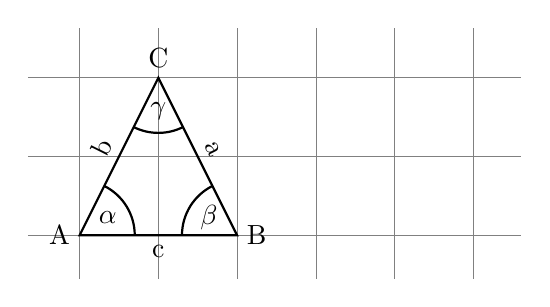
\begin{tikzpicture}[show background grid]
\coordinate (A) at (0,0);
\coordinate (B) at (0:1.6);
\coordinate (C) at (28.955024371859846:2.8);
\draw (A)  (B)    (C)   (A);
\draw[thick,black] (-3,0) coordinate(A) -- node[below,sloped]{c} ++(2,0) coordinate(B) -- node[above,sloped]{a} ++(-1,2) coordinate(C) -- node[above,sloped]{b} cycle; 
\node[left] at (A) {A};
\node[right] at (B) {B};
\node[above] at (C) {C};
\pic [draw,thick, black,angle radius=0.7cm, "$\alpha$"] {angle = B--A--C};
\pic [draw,thick, black,angle radius=0.7cm, "$\beta$"] {angle = C--B--A};
\pic [draw,thick, black,angle radius=0.7cm, "$\gamma$"] {angle = A--C--B};
\end{tikzpicture}
}
&
1b)&
\pbox{\linewidth}{{
Markiere die Planfigure und Konstruiere das Dreieck für folgende Werten:\\
$\begin{aligned}
a&=2,4~cm \\
b&=1,8~cm \\
c&=2,1~cm \\
\end{aligned}$
\tikzstyle{background grid}=[draw, black!15,step=.5cm]
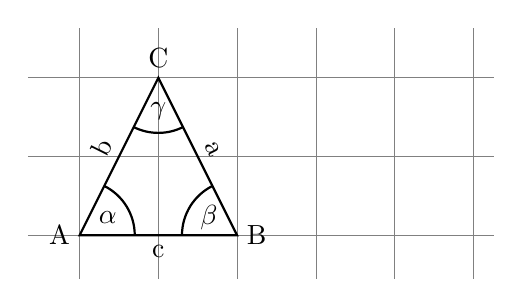
\begin{tikzpicture}[show background grid]
\coordinate (A) at (0,0);
\coordinate (B) at (0:2.1);
\coordinate (C) at (75.52248781407008:1.8);
\draw (A)  (B)    (C)   (A);
\draw[thick,black] (-3,0) coordinate(A) -- node[below,sloped]{c} ++(2,0) coordinate(B) -- node[above,sloped]{a} ++(-1,2) coordinate(C) -- node[above,sloped]{b} cycle; 
\node[left] at (A) {A};
\node[right] at (B) {B};
\node[above] at (C) {C};
\pic [draw,thick, black,angle radius=0.7cm, "$\alpha$"] {angle = B--A--C};
\pic [draw,thick, black,angle radius=0.7cm, "$\beta$"] {angle = C--B--A};
\pic [draw,thick, black,angle radius=0.7cm, "$\gamma$"] {angle = A--C--B};
\end{tikzpicture}
}
\\\hline
1c)&
\pbox{\linewidth}{{
Markiere die Planfigure und Konstruiere das Dreieck für folgende Werten:\\
$\begin{aligned}
a&=2,7~cm \\
b&=2,5~cm \\
c&=2,3~cm \\
\end{aligned}$
\tikzstyle{background grid}=[draw, black!15,step=.5cm]
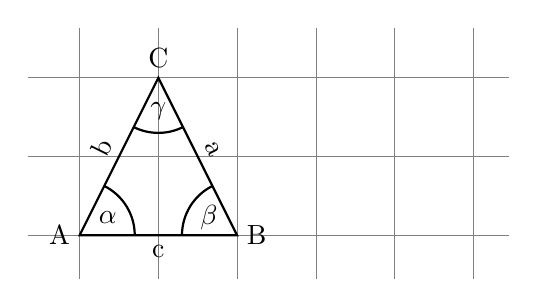
\begin{tikzpicture}[show background grid]
\coordinate (A) at (0,0);
\coordinate (B) at (0:2.3);
\coordinate (C) at (68.31119438185885:2.5);
\draw (A)  (B)    (C)   (A);
\draw[thick,black] (-3,0) coordinate(A) -- node[below,sloped]{c} ++(2,0) coordinate(B) -- node[above,sloped]{a} ++(-1,2) coordinate(C) -- node[above,sloped]{b} cycle; 
\node[left] at (A) {A};
\node[right] at (B) {B};
\node[above] at (C) {C};
\pic [draw,thick, black,angle radius=0.7cm, "$\alpha$"] {angle = B--A--C};
\pic [draw,thick, black,angle radius=0.7cm, "$\beta$"] {angle = C--B--A};
\pic [draw,thick, black,angle radius=0.7cm, "$\gamma$"] {angle = A--C--B};
\end{tikzpicture}
}
&
1d)&
\pbox{\linewidth}{{
Markiere die Planfigure und Konstruiere das Dreieck für folgende Werten:\\
$\begin{aligned}
a&=2~cm \\
b&=2,8~cm \\
c&=2,6~cm \\
\end{aligned}$
\tikzstyle{background grid}=[draw, black!15,step=.5cm]
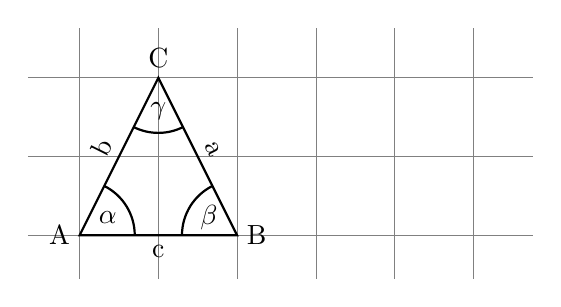
\begin{tikzpicture}[show background grid]
\coordinate (A) at (0,0);
\coordinate (B) at (0:2.6);
\coordinate (C) at (43.27917520057223:2.8);
\draw (A)  (B)    (C)   (A);
\draw[thick,black] (-3,0) coordinate(A) -- node[below,sloped]{c} ++(2,0) coordinate(B) -- node[above,sloped]{a} ++(-1,2) coordinate(C) -- node[above,sloped]{b} cycle; 
\node[left] at (A) {A};
\node[right] at (B) {B};
\node[above] at (C) {C};
\pic [draw,thick, black,angle radius=0.7cm, "$\alpha$"] {angle = B--A--C};
\pic [draw,thick, black,angle radius=0.7cm, "$\beta$"] {angle = C--B--A};
\pic [draw,thick, black,angle radius=0.7cm, "$\gamma$"] {angle = A--C--B};
\end{tikzpicture}
}
\\\hline
2a)&
\pbox{\linewidth}{{
Zeichne die Planfigure und Konstruiere das Dreieck für folgende Werten:\\
$\begin{aligned}
a&=2,6~cm \\
b&=2,4~cm \\
c&=2,3~cm \\
\end{aligned}$
\tikzstyle{background grid}=[draw, black!15,step=.5cm]
\begin{tikzpicture}[show background grid]
\coordinate (A) at (0,0);
\coordinate (B) at (0:2.3);
\coordinate (C) at (67.13339575542875:2.4);
\draw (A)  (B)    (C)   (A);
\node (U) at  (-3,0) {};
\end{tikzpicture}
}
&
2b)&
\pbox{\linewidth}{{
Zeichne die Planfigure und Konstruiere das Dreieck für folgende Werten:\\
$\begin{aligned}
a&=2,2~cm \\
b&=2,5~cm \\
c&=1,6~cm \\
\end{aligned}$
\tikzstyle{background grid}=[draw, black!15,step=.5cm]
\begin{tikzpicture}[show background grid]
\coordinate (A) at (0,0);
\coordinate (B) at (0:1.6);
\coordinate (C) at (60.247789424301345:2.5);
\draw (A)  (B)    (C)   (A);
\node (U) at  (-3,0) {};
\end{tikzpicture}
}
\\\hline
2c)&
\pbox{\linewidth}{{
Zeichne die Planfigure und Konstruiere das Dreieck für folgende Werten:\\
$\begin{aligned}
a&=3~cm \\
b&=1,6~cm \\
c&=2,5~cm \\
\end{aligned}$
\tikzstyle{background grid}=[draw, black!15,step=.5cm]
\begin{tikzpicture}[show background grid]
\coordinate (A) at (0,0);
\coordinate (B) at (0:2.5);
\coordinate (C) at (91.36090272292059:1.6);
\draw (A)  (B)    (C)   (A);
\node (U) at  (-3,0) {};
\end{tikzpicture}
}
&
2d)&
\pbox{\linewidth}{{
Zeichne die Planfigure und Konstruiere das Dreieck für folgende Werten:\\
$\begin{aligned}
a&=2,6~cm \\
b&=2,7~cm \\
c&=3~cm \\
\end{aligned}$
\tikzstyle{background grid}=[draw, black!15,step=.5cm]
\begin{tikzpicture}[show background grid]
\coordinate (A) at (0,0);
\coordinate (B) at (0:3.0);
\coordinate (C) at (53.96554825915242:2.7);
\draw (A)  (B)    (C)   (A);
\node (U) at  (-3,0) {};
\end{tikzpicture}
}
\\\hline
\end{xltabular}
\vspace{0.5cm}
\newpage
\rightline{Datum: 04.12.2024}
\centerline{{\large Lösungen Tägliche Übungen}} 
\vspace{0.5cm}

\begin{xltabular}{\textwidth}{|C{0.75cm}|X|C{0.75cm}|X|}
\arrayrulecolor{black}\hline
1a)&
\begin{adjustbox}{max width=7 cm}
\tikzstyle{background grid}=[draw, black!15,step=.5cm]
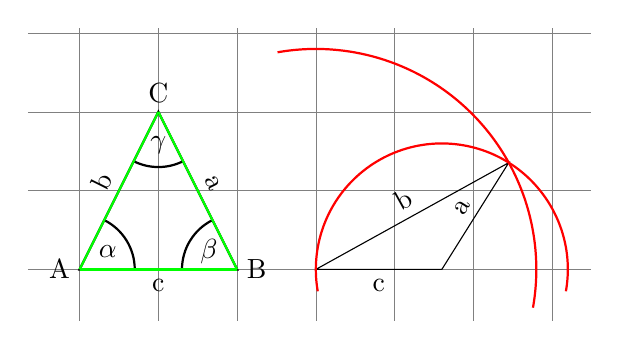
\begin{tikzpicture}[show background grid]
\coordinate (A) at (0,0);
\coordinate (B) at (0:1.6);
\coordinate (C) at (28.955024371859846:2.8);
\draw (A) -- node[below,sloped] {c} (B)   -- node[above,sloped] {a} (C)  -- node[above,sloped] {b} (A);
\draw[thick,red] ($(A)+(-10:2.8)$) arc (-10:100:2.8 cm);
\draw[thick,red] ($(B)+(-10:1.6)$) arc (-10:190:1.6 cm);
\draw[thick,black] (-3,0) coordinate(A) -- node[below,sloped]{c} ++(2,0) coordinate(B) -- node[above,sloped]{a} ++(-1,2) coordinate(C) -- node[above,sloped]{b} cycle; 
\node[left] at (A) {A};
\node[right] at (B) {B};
\node[above] at (C) {C};
\pic [draw,thick, black,angle radius=0.7cm, "$\alpha$"] {angle = B--A--C};
\pic [draw,thick, black,angle radius=0.7cm, "$\beta$"] {angle = C--B--A};
\pic [draw,thick, black,angle radius=0.7cm, "$\gamma$"] {angle = A--C--B};
\draw[thick,green] (B) -- (C);
\draw[thick,green] (A) -- (C);
\draw[thick,green] (A) -- (B);
\end{tikzpicture}
\end{adjustbox}
&
1b)&
\begin{adjustbox}{max width=7 cm}
\tikzstyle{background grid}=[draw, black!15,step=.5cm]
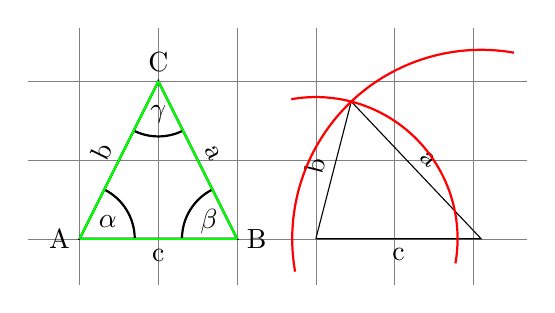
\begin{tikzpicture}[show background grid]
\coordinate (A) at (0,0);
\coordinate (B) at (0:2.1);
\coordinate (C) at (75.52248781407008:1.8);
\draw (A) -- node[below,sloped] {c} (B)   -- node[above,sloped] {a} (C)  -- node[above,sloped] {b} (A);
\draw[thick,red] ($(A)+(-10:1.8)$) arc (-10:100:1.8 cm);
\draw[thick,red] ($(B)+(80:2.4)$) arc (80:190:2.4 cm);
\draw[thick,black] (-3,0) coordinate(A) -- node[below,sloped]{c} ++(2,0) coordinate(B) -- node[above,sloped]{a} ++(-1,2) coordinate(C) -- node[above,sloped]{b} cycle; 
\node[left] at (A) {A};
\node[right] at (B) {B};
\node[above] at (C) {C};
\pic [draw,thick, black,angle radius=0.7cm, "$\alpha$"] {angle = B--A--C};
\pic [draw,thick, black,angle radius=0.7cm, "$\beta$"] {angle = C--B--A};
\pic [draw,thick, black,angle radius=0.7cm, "$\gamma$"] {angle = A--C--B};
\draw[thick,green] (B) -- (C);
\draw[thick,green] (A) -- (C);
\draw[thick,green] (A) -- (B);
\end{tikzpicture}
\end{adjustbox}
\\\hline
1c)&
\begin{adjustbox}{max width=7 cm}
\tikzstyle{background grid}=[draw, black!15,step=.5cm]
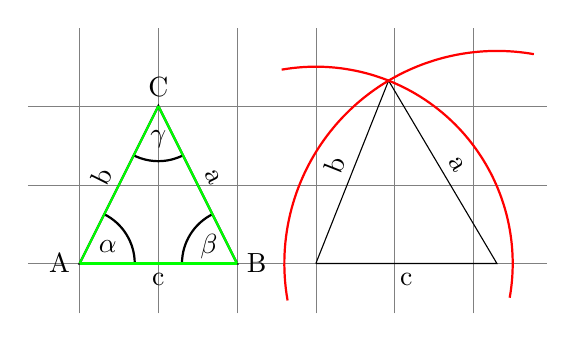
\begin{tikzpicture}[show background grid]
\coordinate (A) at (0,0);
\coordinate (B) at (0:2.3);
\coordinate (C) at (68.31119438185885:2.5);
\draw (A) -- node[below,sloped] {c} (B)   -- node[above,sloped] {a} (C)  -- node[above,sloped] {b} (A);
\draw[thick,red] ($(A)+(-10:2.5)$) arc (-10:100:2.5 cm);
\draw[thick,red] ($(B)+(80:2.7)$) arc (80:190:2.7 cm);
\draw[thick,black] (-3,0) coordinate(A) -- node[below,sloped]{c} ++(2,0) coordinate(B) -- node[above,sloped]{a} ++(-1,2) coordinate(C) -- node[above,sloped]{b} cycle; 
\node[left] at (A) {A};
\node[right] at (B) {B};
\node[above] at (C) {C};
\pic [draw,thick, black,angle radius=0.7cm, "$\alpha$"] {angle = B--A--C};
\pic [draw,thick, black,angle radius=0.7cm, "$\beta$"] {angle = C--B--A};
\pic [draw,thick, black,angle radius=0.7cm, "$\gamma$"] {angle = A--C--B};
\draw[thick,green] (B) -- (C);
\draw[thick,green] (A) -- (C);
\draw[thick,green] (A) -- (B);
\end{tikzpicture}
\end{adjustbox}
&
1d)&
\begin{adjustbox}{max width=7 cm}
\tikzstyle{background grid}=[draw, black!15,step=.5cm]
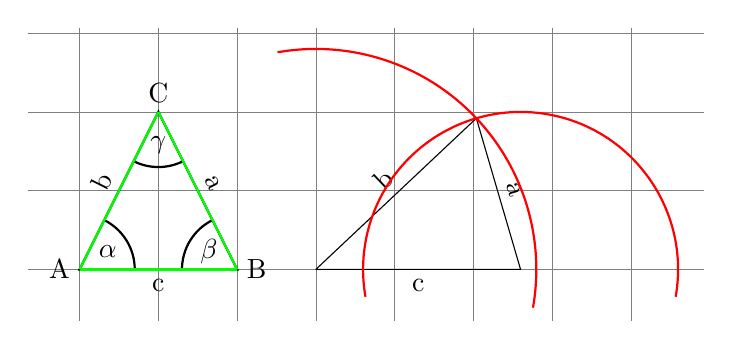
\begin{tikzpicture}[show background grid]
\coordinate (A) at (0,0);
\coordinate (B) at (0:2.6);
\coordinate (C) at (43.27917520057223:2.8);
\draw (A) -- node[below,sloped] {c} (B)   -- node[above,sloped] {a} (C)  -- node[above,sloped] {b} (A);
\draw[thick,red] ($(A)+(-10:2.8)$) arc (-10:100:2.8 cm);
\draw[thick,red] ($(B)+(-10:2.0)$) arc (-10:190:2.0 cm);
\draw[thick,black] (-3,0) coordinate(A) -- node[below,sloped]{c} ++(2,0) coordinate(B) -- node[above,sloped]{a} ++(-1,2) coordinate(C) -- node[above,sloped]{b} cycle; 
\node[left] at (A) {A};
\node[right] at (B) {B};
\node[above] at (C) {C};
\pic [draw,thick, black,angle radius=0.7cm, "$\alpha$"] {angle = B--A--C};
\pic [draw,thick, black,angle radius=0.7cm, "$\beta$"] {angle = C--B--A};
\pic [draw,thick, black,angle radius=0.7cm, "$\gamma$"] {angle = A--C--B};
\draw[thick,green] (B) -- (C);
\draw[thick,green] (A) -- (C);
\draw[thick,green] (A) -- (B);
\end{tikzpicture}
\end{adjustbox}
\\\hline
2a)&
\begin{adjustbox}{max width=7 cm}
\tikzstyle{background grid}=[draw, black!15,step=.5cm]
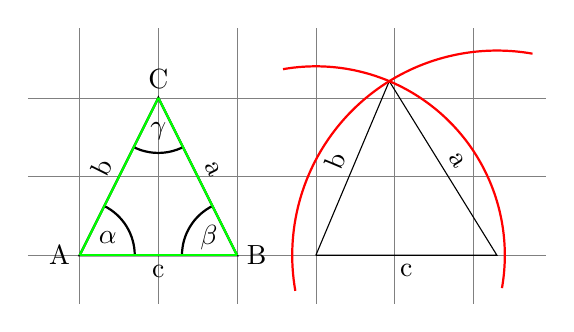
\begin{tikzpicture}[show background grid]
\coordinate (A) at (0,0);
\coordinate (B) at (0:2.3);
\coordinate (C) at (67.13339575542875:2.4);
\draw (A) -- node[below,sloped] {c} (B)   -- node[above,sloped] {a} (C)  -- node[above,sloped] {b} (A);
\draw[thick,red] ($(A)+(-10:2.4)$) arc (-10:100:2.4 cm);
\draw[thick,red] ($(B)+(80:2.6)$) arc (80:190:2.6 cm);
\draw[thick,black] (-3,0) coordinate(A) -- node[below,sloped]{c} ++(2,0) coordinate(B) -- node[above,sloped]{a} ++(-1,2) coordinate(C) -- node[above,sloped]{b} cycle; 
\node[left] at (A) {A};
\node[right] at (B) {B};
\node[above] at (C) {C};
\pic [draw,thick, black,angle radius=0.7cm, "$\alpha$"] {angle = B--A--C};
\pic [draw,thick, black,angle radius=0.7cm, "$\beta$"] {angle = C--B--A};
\pic [draw,thick, black,angle radius=0.7cm, "$\gamma$"] {angle = A--C--B};
\draw[thick,green] (B) -- (C);
\draw[thick,green] (A) -- (C);
\draw[thick,green] (A) -- (B);
\end{tikzpicture}
\end{adjustbox}
&
2b)&
\begin{adjustbox}{max width=7 cm}
\tikzstyle{background grid}=[draw, black!15,step=.5cm]
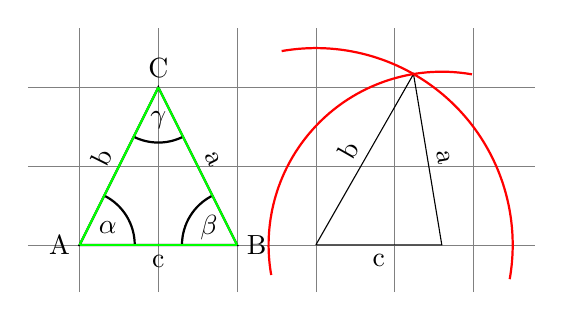
\begin{tikzpicture}[show background grid]
\coordinate (A) at (0,0);
\coordinate (B) at (0:1.6);
\coordinate (C) at (60.247789424301345:2.5);
\draw (A) -- node[below,sloped] {c} (B)   -- node[above,sloped] {a} (C)  -- node[above,sloped] {b} (A);
\draw[thick,red] ($(A)+(-10:2.5)$) arc (-10:100:2.5 cm);
\draw[thick,red] ($(B)+(80:2.2)$) arc (80:190:2.2 cm);
\draw[thick,black] (-3,0) coordinate(A) -- node[below,sloped]{c} ++(2,0) coordinate(B) -- node[above,sloped]{a} ++(-1,2) coordinate(C) -- node[above,sloped]{b} cycle; 
\node[left] at (A) {A};
\node[right] at (B) {B};
\node[above] at (C) {C};
\pic [draw,thick, black,angle radius=0.7cm, "$\alpha$"] {angle = B--A--C};
\pic [draw,thick, black,angle radius=0.7cm, "$\beta$"] {angle = C--B--A};
\pic [draw,thick, black,angle radius=0.7cm, "$\gamma$"] {angle = A--C--B};
\draw[thick,green] (B) -- (C);
\draw[thick,green] (A) -- (C);
\draw[thick,green] (A) -- (B);
\end{tikzpicture}
\end{adjustbox}
\\\hline
2c)&
\begin{adjustbox}{max width=7 cm}
\tikzstyle{background grid}=[draw, black!15,step=.5cm]
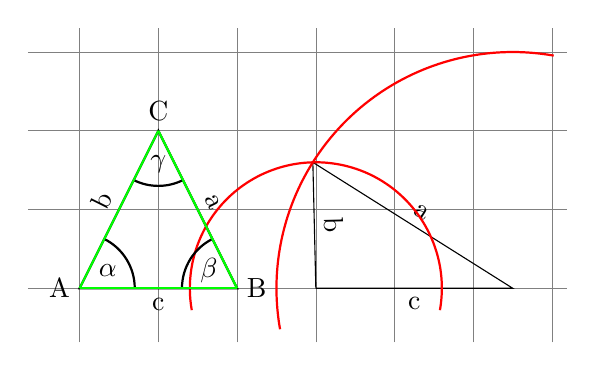
\begin{tikzpicture}[show background grid]
\coordinate (A) at (0,0);
\coordinate (B) at (0:2.5);
\coordinate (C) at (91.36090272292059:1.6);
\draw (A) -- node[below,sloped] {c} (B)   -- node[above,sloped] {a} (C)  -- node[above,sloped] {b} (A);
\draw[thick,red] ($(A)+(-10:1.6)$) arc (-10:190:1.6 cm);
\draw[thick,red] ($(B)+(80:3.0)$) arc (80:190:3.0 cm);
\draw[thick,black] (-3,0) coordinate(A) -- node[below,sloped]{c} ++(2,0) coordinate(B) -- node[above,sloped]{a} ++(-1,2) coordinate(C) -- node[above,sloped]{b} cycle; 
\node[left] at (A) {A};
\node[right] at (B) {B};
\node[above] at (C) {C};
\pic [draw,thick, black,angle radius=0.7cm, "$\alpha$"] {angle = B--A--C};
\pic [draw,thick, black,angle radius=0.7cm, "$\beta$"] {angle = C--B--A};
\pic [draw,thick, black,angle radius=0.7cm, "$\gamma$"] {angle = A--C--B};
\draw[thick,green] (B) -- (C);
\draw[thick,green] (A) -- (C);
\draw[thick,green] (A) -- (B);
\end{tikzpicture}
\end{adjustbox}
&
2d)&
\begin{adjustbox}{max width=7 cm}
\tikzstyle{background grid}=[draw, black!15,step=.5cm]
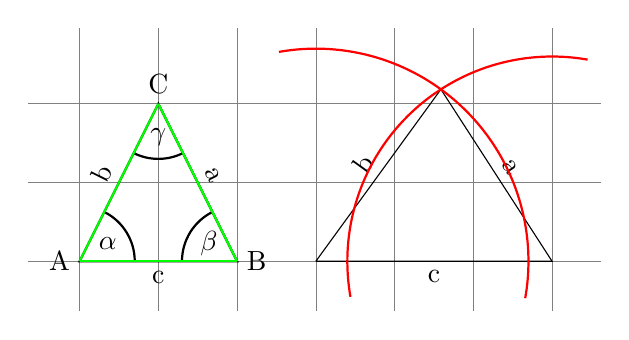
\begin{tikzpicture}[show background grid]
\coordinate (A) at (0,0);
\coordinate (B) at (0:3.0);
\coordinate (C) at (53.96554825915242:2.7);
\draw (A) -- node[below,sloped] {c} (B)   -- node[above,sloped] {a} (C)  -- node[above,sloped] {b} (A);
\draw[thick,red] ($(A)+(-10:2.7)$) arc (-10:100:2.7 cm);
\draw[thick,red] ($(B)+(80:2.6)$) arc (80:190:2.6 cm);
\draw[thick,black] (-3,0) coordinate(A) -- node[below,sloped]{c} ++(2,0) coordinate(B) -- node[above,sloped]{a} ++(-1,2) coordinate(C) -- node[above,sloped]{b} cycle; 
\node[left] at (A) {A};
\node[right] at (B) {B};
\node[above] at (C) {C};
\pic [draw,thick, black,angle radius=0.7cm, "$\alpha$"] {angle = B--A--C};
\pic [draw,thick, black,angle radius=0.7cm, "$\beta$"] {angle = C--B--A};
\pic [draw,thick, black,angle radius=0.7cm, "$\gamma$"] {angle = A--C--B};
\draw[thick,green] (B) -- (C);
\draw[thick,green] (A) -- (C);
\draw[thick,green] (A) -- (B);
\end{tikzpicture}
\end{adjustbox}
\\\hline
\end{xltabular}
\vspace{0.5cm}
\end{document}